\documentclass[11pt]{article}
\usepackage{graphicx}
\usepackage[margin=2.5cm]{geometry}
\usepackage{tikz}
\usepackage{indentfirst}
\usepackage{tabularx}
\usepackage{listingsutf8}
\usepackage{color}
\usepackage{hyperref}
\usepackage{float}
\usepackage[portuguese]{babel}

\graphicspath{{./images/}{./screenshots/}}

\def\checkmark{\tikz\fill[scale=0.4](0,.35) -- (.25,0) -- (1,.7) -- (.25,.15) -- cycle;} 
\setlength{\parskip}{0.5em}

\renewcommand{\lstlistingname}{Código}
\renewcommand{\lstlistlistingname}{Pedaços de Código}

\definecolor{dkgreen}{rgb}{0,0.6,0}
\definecolor{gray}{rgb}{0.5,0.5,0.5}
\definecolor{mauve}{rgb}{0.58,0,0.82}

\hypersetup{
	colorlinks=false,
	linktoc=all,
	hidelinks,
}

\lstdefinelanguage{Kotlin}{
	comment=[l]{//},
	commentstyle={\color{gray}\ttfamily},
	emph={filter, first, firstOrNull, forEach, lazy, map, mapNotNull, println},
	emphstyle={\color{OrangeRed}},
	identifierstyle=\color{black},
	keywords={!in, !is, abstract, actual, annotation, as, as?, break, by, catch, class, companion, const, constructor, continue, crossinline, data, delegate, do, dynamic, else, enum, expect, external, false, field, file, final, finally, for, fun, get, if, import, in, infix, init, inline, inner, interface, internal, is, lateinit, noinline, null, object, open, operator, out, override, package, param, private, property, protected, public, receiveris, reified, return, return@, sealed, set, setparam, super, suspend, tailrec, this, throw, true, try, typealias, typeof, val, var, vararg, when, where, while},
	keywordstyle={\color{NavyBlue}\bfseries},
	morecomment=[s]{/*}{*/},
	morestring=[b]",
	morestring=[s]{"""*}{*"""},
	ndkeywords={@Deprecated, @JvmField, @JvmName, @JvmOverloads, @JvmStatic, @JvmSynthetic, Array, Byte, Double, Float, Int, Integer, Iterable, Long, Runnable, Short, String, Any, Unit, Nothing},
	ndkeywordstyle={\color{BurntOrange}\bfseries},
	sensitive=true,
	stringstyle={\color{ForestGreen}\ttfamily},
}

\lstset{
	belowcaptionskip=1\baselineskip,
	captionpos=b,
	frame=tb,
	language=Kotlin,
	aboveskip=3mm,
	belowskip=3mm,
	showstringspaces=false,
	columns=flexible,
	basicstyle={\small\ttfamily},
	numbers=none,
	numberstyle=\tiny\color{gray},
	keywordstyle=\color{blue},
	commentstyle=\color{dkgreen},
	stringstyle=\color{mauve},
	breaklines=true,
	breakatwhitespace=true,
	tabsize=3,
	inputencoding=utf8,
	extendedchars=true,
	literate={á}{{\'a}}1 {ã}{{\~a}}1 {à}{{\`a} }1 {Ã}{{\~A}}1 {ó}{{\'o}}1 {Ó}{{\'O}}1 {Í}{{\'I}}1 {í}{{\'i}}1 {é}{{\'e}}1 {ç}{{\c{c}}}1 {Ç}{{\c{C}}}1 {ú}{{\'u}}1 {õ}{{\~o}}1
}

\begin{document}
	\begin{titlepage}
		\begin{center}
			
\includegraphics[width=0.6\textwidth]{logo-isec}
			
			\vspace*{\fill}
			
			
\includegraphics[width=0.4\textwidth]{icon-airbnb}
			
			\Huge
			\textbf{airbnb}
			
			\huge
			Relatório de Execução do Trabalho Prático
			
			\vspace{2cm}
			
			\Large
			\textbf{
				Ângelo Paiva, 2019129023 \\
				Bruno Teixeira, 2019100036
			}
			
			\vfill
			\vspace*{\fill}
			
			\normalsize
			Programação Web \\
			Licenciatura de Engenharia Informática \\
			20 de janeiro de 2022		
		\end{center}
	\end{titlepage}
	
	\tableofcontents
	\pagebreak
	
	\large
	\section{Introdução}
	\normalsize
	
	Neste trabalho foi realizado um website para arrendamento de espaços / casas.
	
	Este relatório irá explicar a implementação, a razão por trás das decisões que foram tomadas e o caminho até à solução entregue.
	

    \large
    \section{Descrição do tema abordado}
    \normalsize
    
    Neste trabalho foi disponibilizada uma plataforma web no modelo SaaS que permite a pessoas com espaços / casas alugar este espaços.
    
    A plataforma foi dividida em quatro partes principais: a área de administração (onde existe apenas um utilizador com acesso), a área de gerentes (ou managers, como chamamos), a área de trabalhadores (ou employees, como chamamos) e a área de cliente (ou customer, como chamamos).
    
    Uma pessoa que pretenda usar o site pode registar-se de duas maneiras: como cliente ou como gerente. Um cliente apenas poderá alugar espaços e deixar reviews, enquanto que o gerente poderá registar espaços que pretende dar a alugar no site, podendo registar novos utilizados na plataforma para trabalharem para ele, ou seja, trabalhadores.
    
    O gerente terá acesso a uma lista dos espaços que tem registados no site, bem como os seus trabalhadores.
    
    O cliente e o utilizador anónimo podem ver o catálogo de todos os espaços / casas disponíveis para alugar, mas apenas o cliente poderá fazer um pedido de aluguer, que poderá ser aceite ou rejeitado pelo manager que registou a acomodação ou um trabalhador que este associou à mesma.
    
    O administrador é um utilizador que existe por defeito na base de dados e tem acesso a tudo menos informação sensível.
    

    \large
    \section{Descrição das regras e relações de modelos}
    \normalsize


    \subsection{Modelo dos Accomodations}
    \normalsize
    
    Este modelo foi criado de modo a representar um alojamento. Para isso foram criados alguns atributos, como por exemplo a descrição do mesmo, a sua categoria, as datas de disponibilidade e o preço por noite.\\
    Depois foi tambem utilizado uma lista de \textbf{AccomodationImages} que representa as imagens que estão associadas a um certo alojamento e uma lista de \textbf{Bookings} uma vez que a mesma vai ser reservada por alguem.\\
    Para fazer a gestão do alojamento, foram criados mais dois atributos, um que faz referência ao \textbf{Manager} que criou o alojamento e outro que faz referência ao \textbf{Employee} que gere o mesmo.
    
    
    \subsection{Modelo dos AccomodationImages}
    \normalsize
    
    Este modelo foi utilizado para guardar informações relativas às imagens, imagens estas que fazem parte de um alojamento. Por fim foi criado um objeto do tipo \textbf{Accomodation} para fazermos a relação entre alojamentos e imagens.
    
    
    \subsection{Modelo dos Bookings}
    \normalsize
    
    O modelo dos \textbf{Bookings} representa uma reserva feita por um \textbf{Customer}, por isso lá, contem toda a informação precisa para ser feita essa tal reserva. Também foi feita a relação com o alojamento, com um cliente e com o empregado que vai aceitar/recusar a reserva.
    
    
    \subsection{Modelo das Categories}
    \normalsize
    
    Aqui encontram-se as categorias referentes a um alojamento, logo, existe aqui uma lista de alojamentos, uma vez que uma categoria pode ter vários alojamentos, mas um alojamento apenas tem uma categoria. O único utilizador que manipula este modelo é o Administrador da plataforma.
    
    
    \subsection{Modelo dos Customers}
    \normalsize
    
    Este modelo é usado para definir o que é um cliente, ou seja, ao ser criado um cliente, ele é criado a partir do \textbf{ApplicationUser} no entanto ao mesmo tempo é criado um objeto do tipo \textbf{Customer} e lá dentro contem um \textbf{public ApplicationUser ApplicationUser} fazendo então referência ao objeto que foi criado na tabela \textbf{dbo.AspNetUsers}.\\
    Este cliente tem tambem uma lista de avaliações (\textbf{AccomodationRatings}) e uma lista de reservas  (\textbf{Bookings}) para assim haver relação com os outros modelos.
    
    
    \subsection{Modelo dos Managers}
    \normalsize
    
    Aqui continua a existir a relação com o \textbf{ApplicationUser}, acrescentando o facto que aqui existe uma lista de empregados (\textbf{Employees}) e uma lista de alojamentos (\textbf{Accomodations}), sendo que estas listas são sempre precisas para que quando fosse feito o \textbf{Add-Migration} fossem aplicadas as devidas relações entre modelos. 
    
    
    \subsection{Modelo dos Employees}
    \normalsize
    
    Um empregado é então gerido por um gestor (\textbf{Manager}), tem uma lista de reservas atribuidas a si (\textbf{Bookings}) e tem tambem uma lista de alojamentos (\textbf{Accomodations}) atribuida a si. Por fim, mais uma vez aqui existe um \textbf{ApplicationUser} para haver sempre facilidade de manipular duas tabelas diferentes e haver relações entre ambas (relação entre a tabela dbo.AspNetUsers e tabela Employees).
    
    
    \subsection{Modelo dos Admins}
    \normalsize
    
    Aqui foi apenas feita a relação com o \textbf{ApplicationUser} mais uma vez para haver relação entre duas tabelas diferentes e para que fosse muito mais fácil aplicar qualquer tipo de \emph{queries}.
    
    
    \large
    \section{Funcionalidades implementadas}
    \normalsize
    
    \begin{center}
    	\begin{tabularx}{\textwidth}{ |X|c|c|c| }
    		\hline
    		\textbf{Componente do Trabalho} & \textbf{Realizado} \\ \hline
    		Autenticação com recurso a ASP.NET Core Identity & \checkmark \\ \hline
    		Recuperação de password & X \\ \hline
    		Base de Dados com recurso a SQLServer (abordagem Code First) & \checkmark \\ \hline
    		Utilizadores (anónimo, cliente, gestor, funcionário, administrador) & \checkmark \\ \hline
    		Utilizadores Registados - login & \checkmark \\ \hline
    		Utilizadores Registados - alterar informação pessoal & \checkmark \\ \hline
    		Anónimo - ver catálogo, registar como cliente ou gestor & \checkmark \\ \hline
    		Cliente - ver catálogo, efetuar reserva, deixar avaliações, ter acesso ao histórico de reservas e avaliações & \checkmark \\ \hline
    		Gestor - criar e gerir funcionários, gestão do portfólio de imóveis, ver avaliações dos imóveis & \checkmark \\ \hline
    		Gestor - definir checklist, avaliar clientes & X \\ \hline
    		Funcionário - gerir reservas & \checkmark \\ \hline
    		Funcionário - analisar cliente para aceitar ou rejeitar o seu pedido de reserva, entregar espaço ao cliente (checklist), receber o espaço do cliente (checklist) & Parcialmente \\ \hline
    		Administrador - gestão de empresas / proprietários, gestão de clientes, gestão de espaços/alojamentos, ver catálogo de espaços disponibilizados & \checkmark \\ \hline
    	\end{tabularx}
    \end{center}


    \large
    \section{Dados de acesso}
	\normalsize        
	\begin{tabular}{ r|c|c| }
		\multicolumn{1}{r}{}
		&  \multicolumn{1}{c}{Email}
		& \multicolumn{1}{c}{Password} \\
		\cline{2-3}
		& admin@airbnb.pt & 1qazZAQ! \\
		\cline{2-3}
		& manager1@isec.pt & 1qazZAQ! \\
		\cline{2-3}
		& manager2@ipc.pt & 1qazZAQ! \\
		\cline{2-3}
		& employee1@isec.pt & 1qazZAQ! \\
		\cline{2-3}
		& employee2@isec.pt & 1qazZAQ! \\
		\cline{2-3}
		& employee1@ipc.pt & 1qazZAQ! \\
		\cline{2-3}
		& employee2@ipc.pt & 1qazZAQ! \\
		\cline{2-3}
		& angelocustomer@angelo.pt & 1qazZAQ! \\
		\cline{2-3}
		& brunocustomer@bruno.pt & 1qazZAQ! \\
		\cline{2-3}
		& teixeiracustomer@teixeira.pt & 1qazZAQ! \\
		\cline{2-3}
		& paivacustomer@paiva.pt & 1qazZAQ! \\
		\cline{2-3}
	\end{tabular}

	
	\newpage
	\vfill

    \large
    \section{Vistas}
    \normalsize
    
    \begin{figure}[!ht]
    	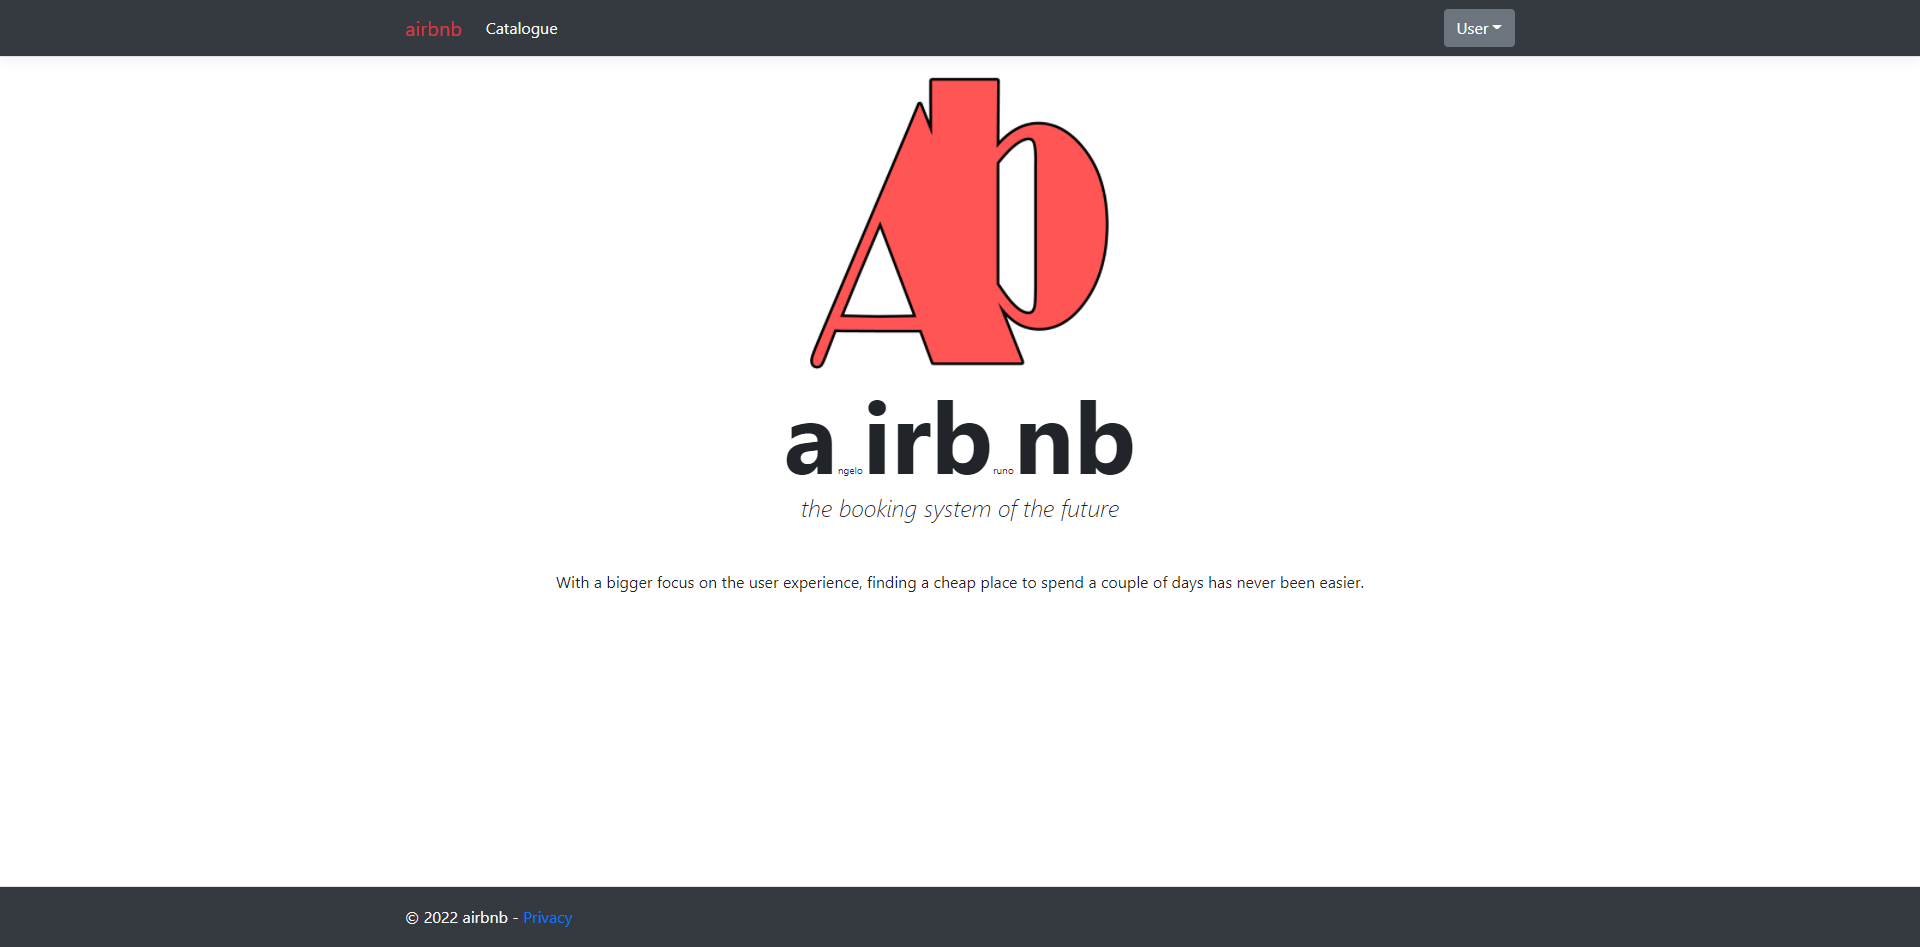
\includegraphics[width=0.95\textwidth,height=0.88\textheight,keepaspectratio]{home-anonymous}
    	\centering
    	\caption{Utilizador Anónimo - Home Page}
    	\label{fig:anonymous-home-page}
    \end{figure}

    \begin{figure}[!ht]
		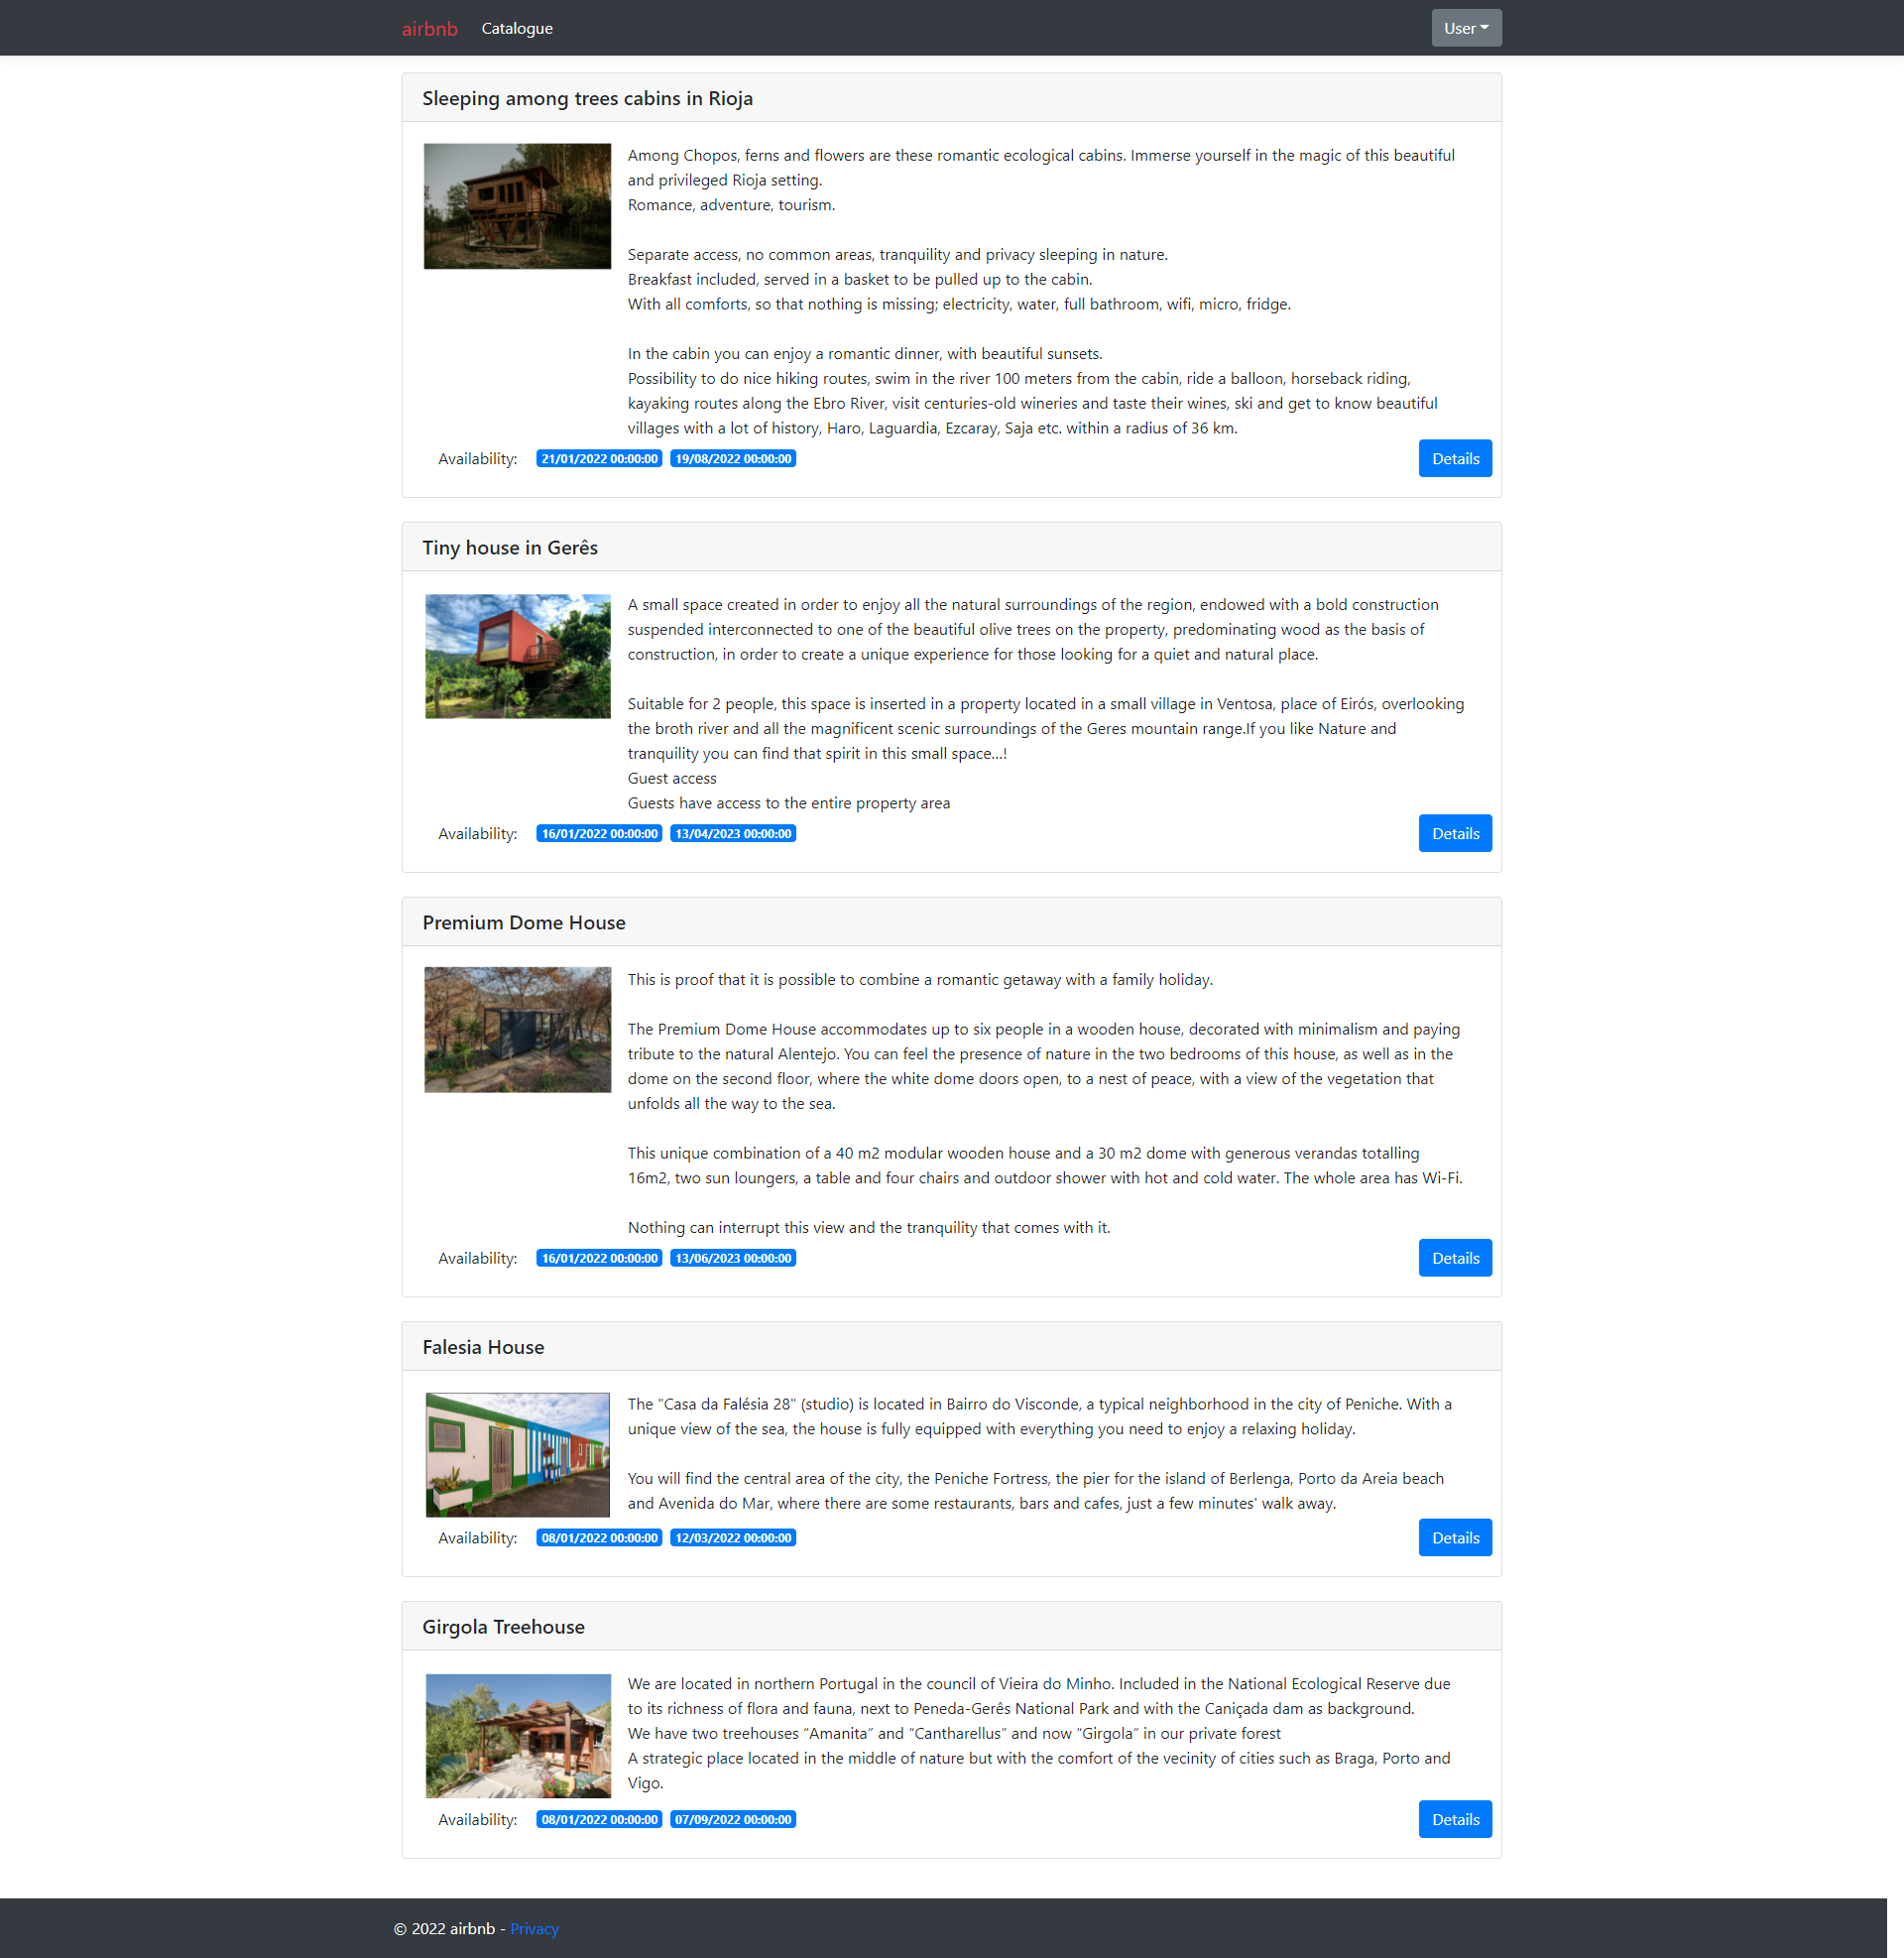
\includegraphics[width=0.95\textwidth,height=0.88\textheight,keepaspectratio]{catalogue-anonymous}
		\centering
		\caption{Utilizador Anónimo - Catálogo}
		\label{fig:anonymous-catalogue}
	\end{figure}

	\begin{figure}[!ht]
		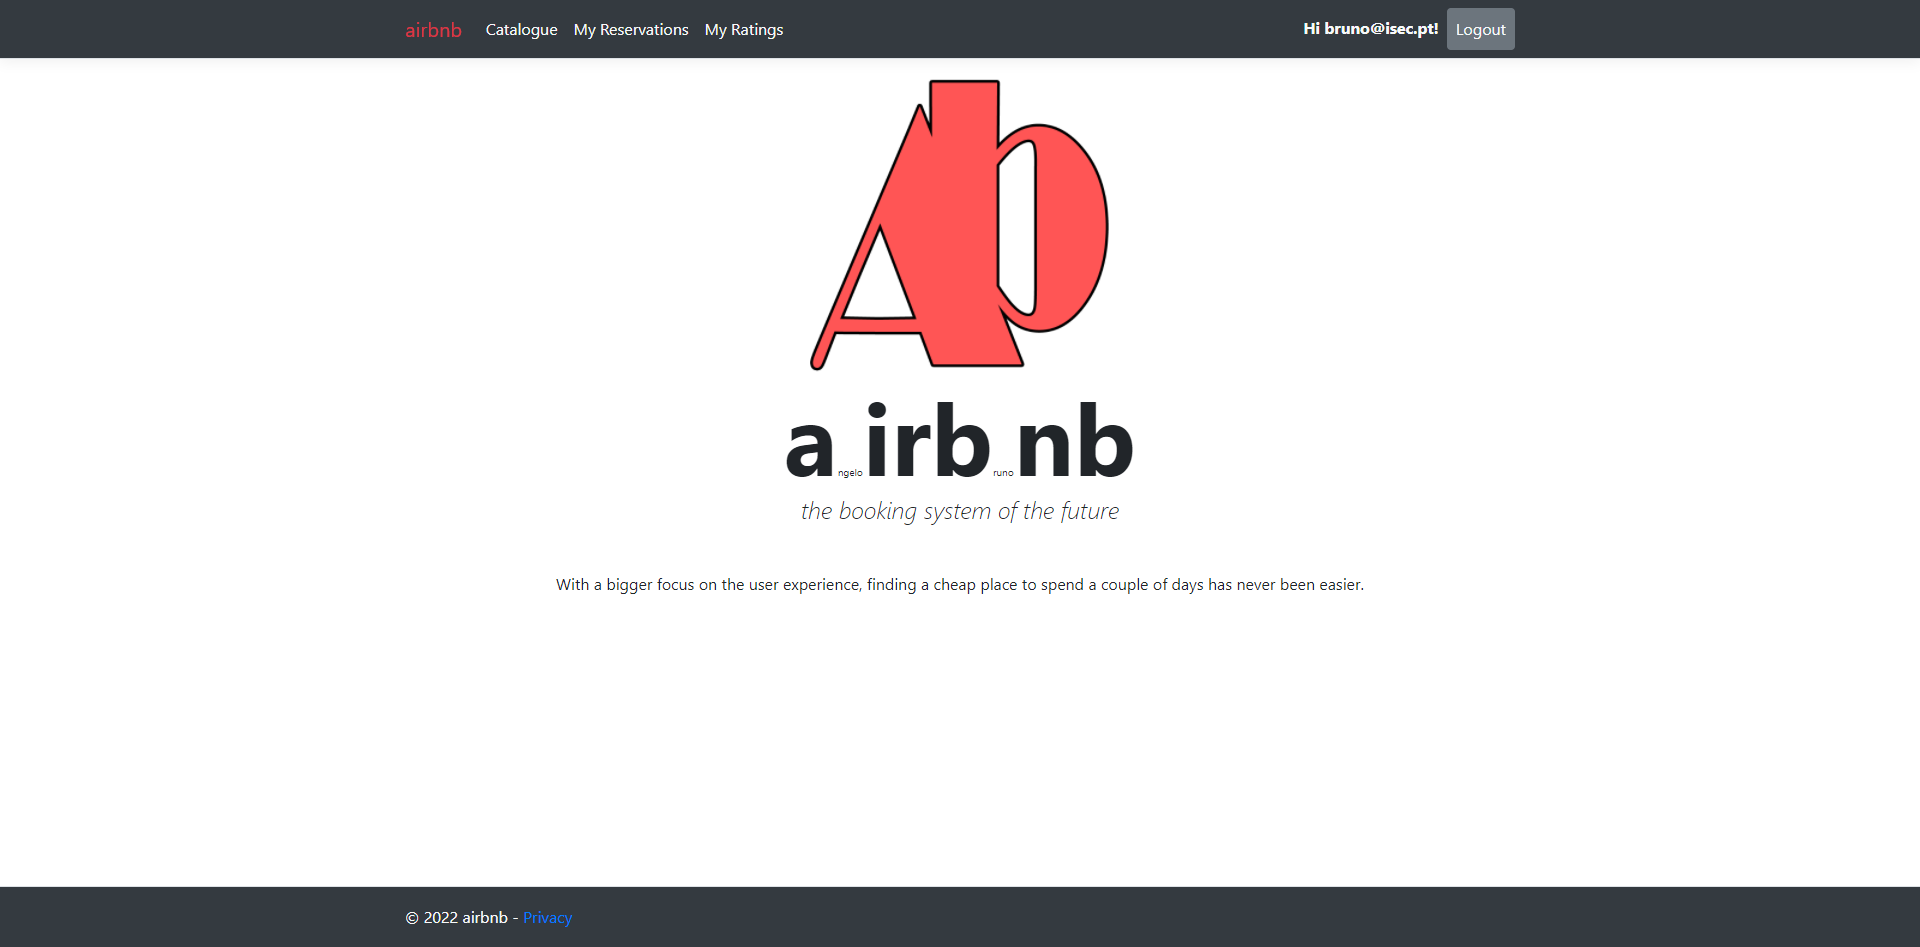
\includegraphics[width=0.95\textwidth,height=0.88\textheight,keepaspectratio]{home-customer}
		\centering
		\caption{Customer - Home Page}
		\label{fig:customer-home-page}
	\end{figure}
	
	\begin{figure}[!ht]
		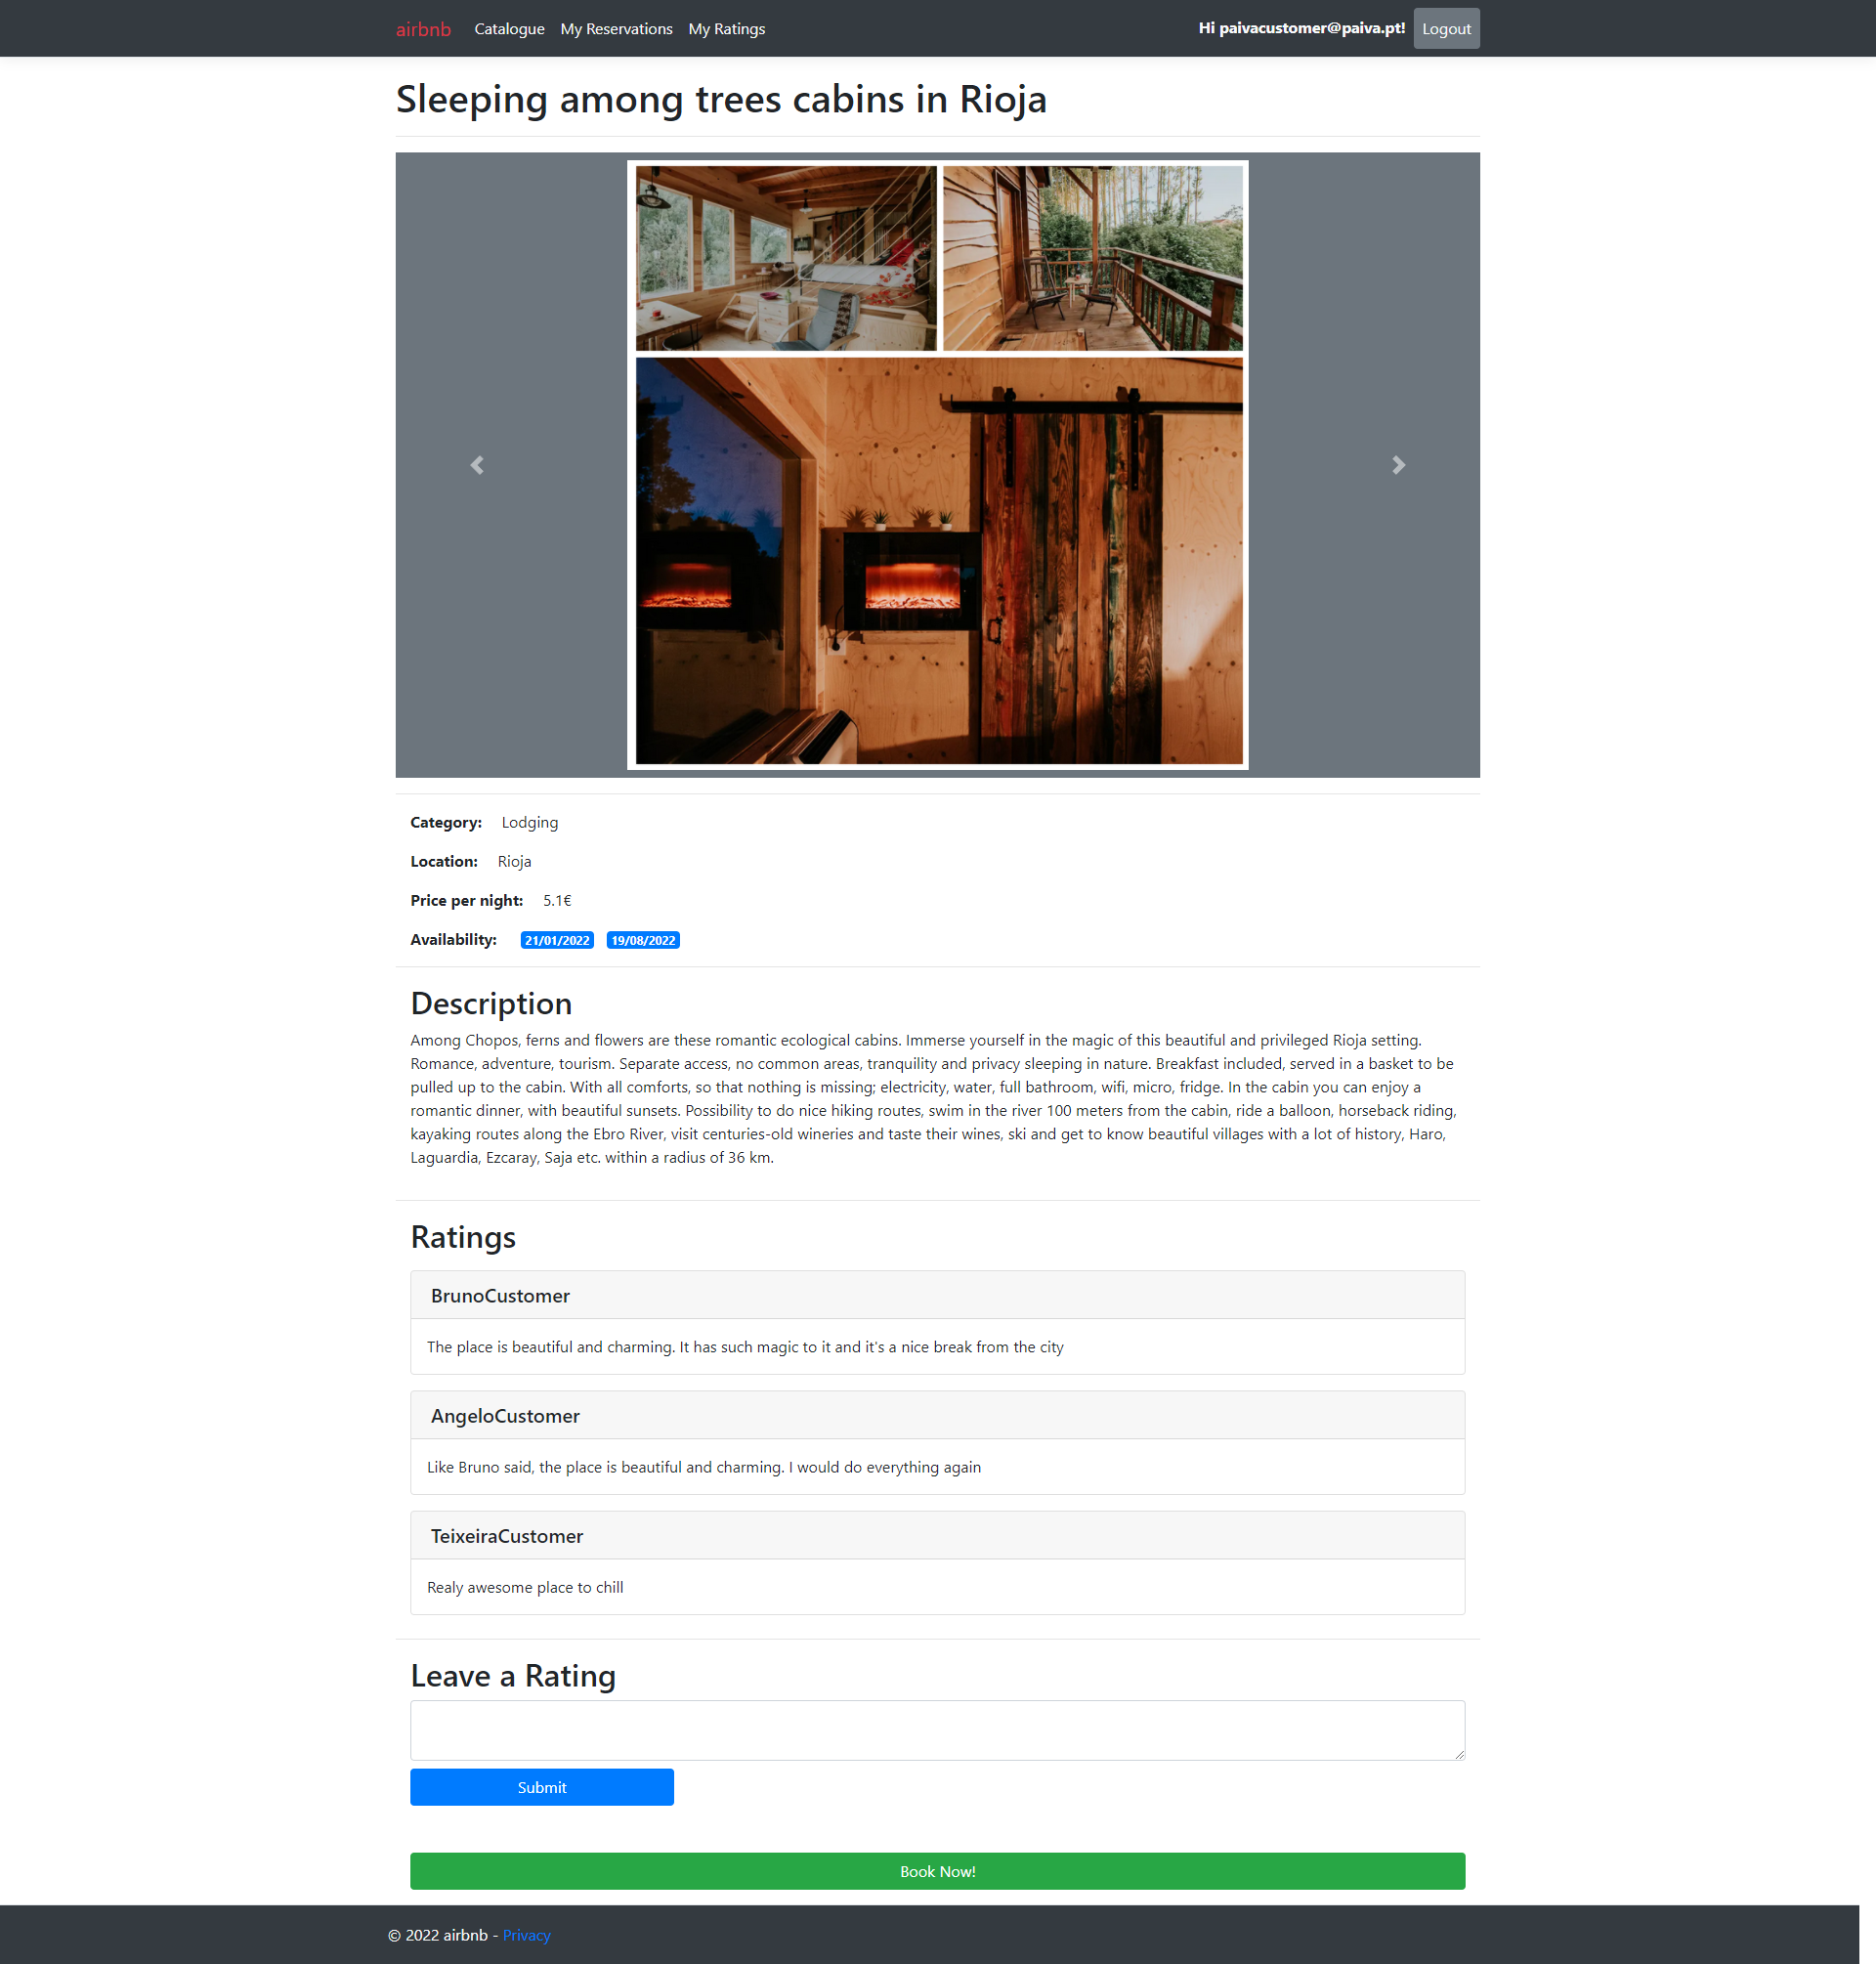
\includegraphics[width=0.95\textwidth,height=0.88\textheight,keepaspectratio]{accommodation-customer}
		\centering
		\caption{Customer - Accommodation}
		\label{fig:customer-accommodation}
	\end{figure}

	\begin{figure}[!ht]
		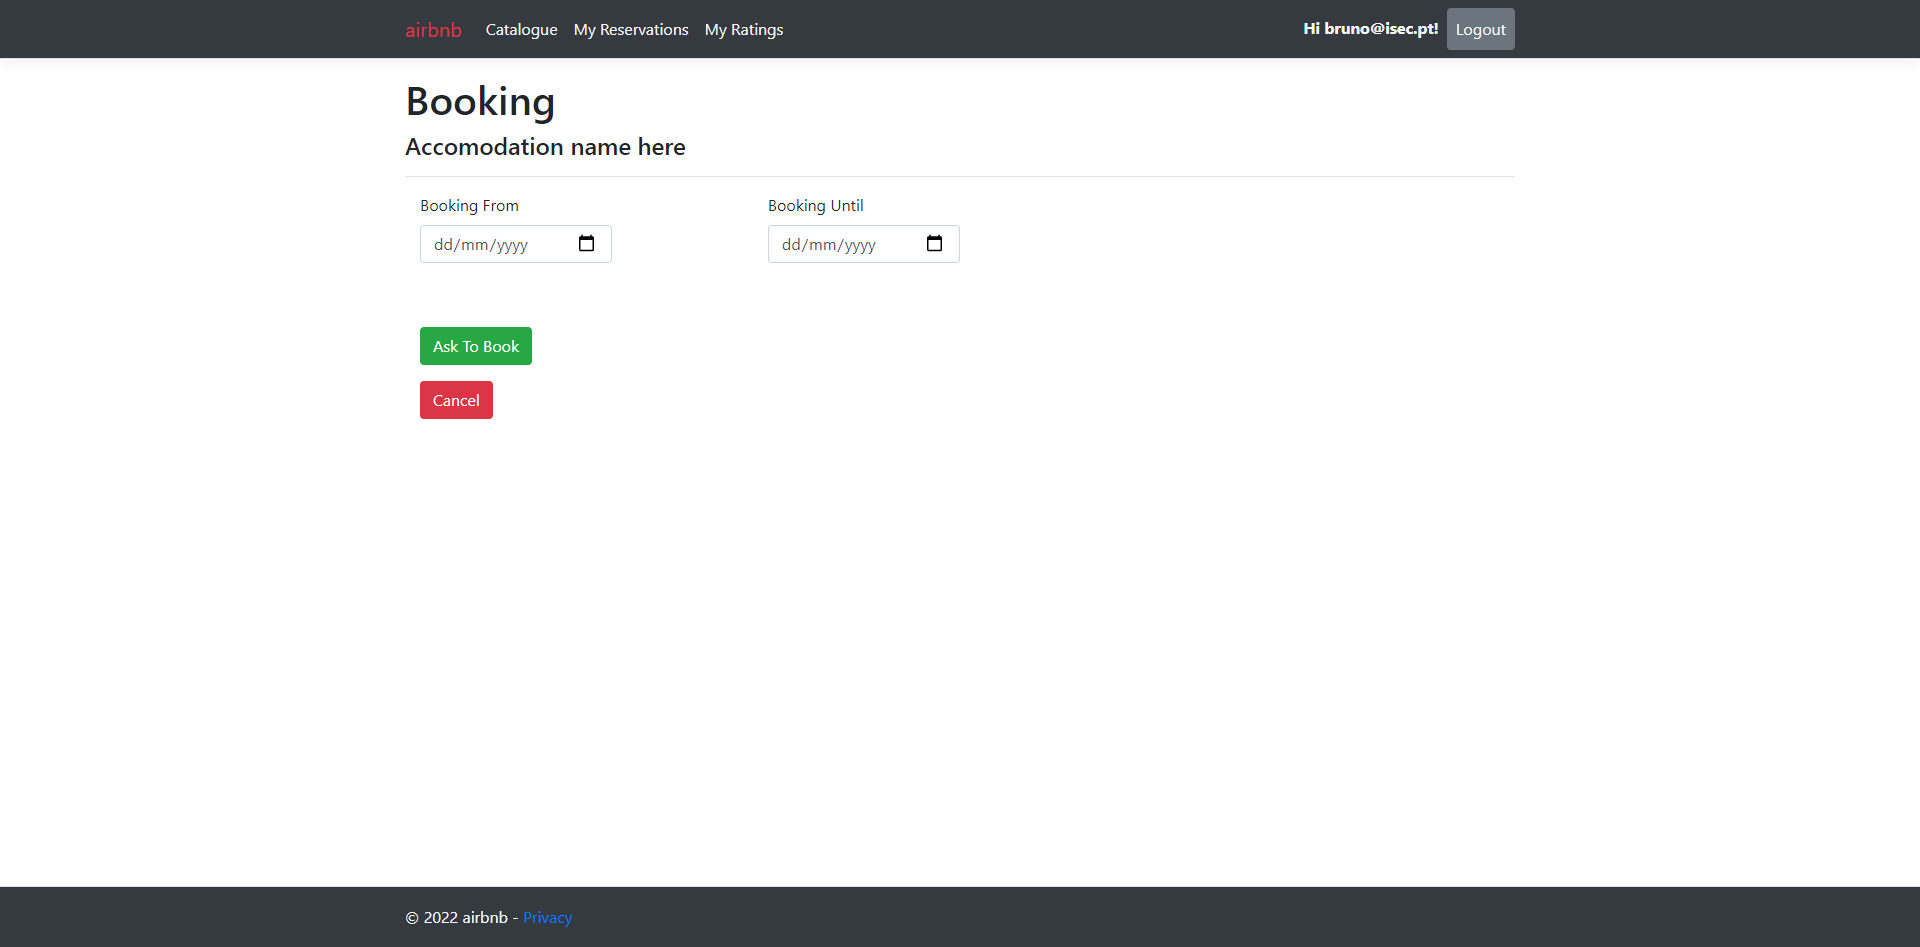
\includegraphics[width=0.95\textwidth,height=0.88\textheight,keepaspectratio]{booking-customer}
		\centering
		\caption{Customer - Booking}
		\label{fig:customer-booking}
	\end{figure}

	\begin{figure}[!ht]
		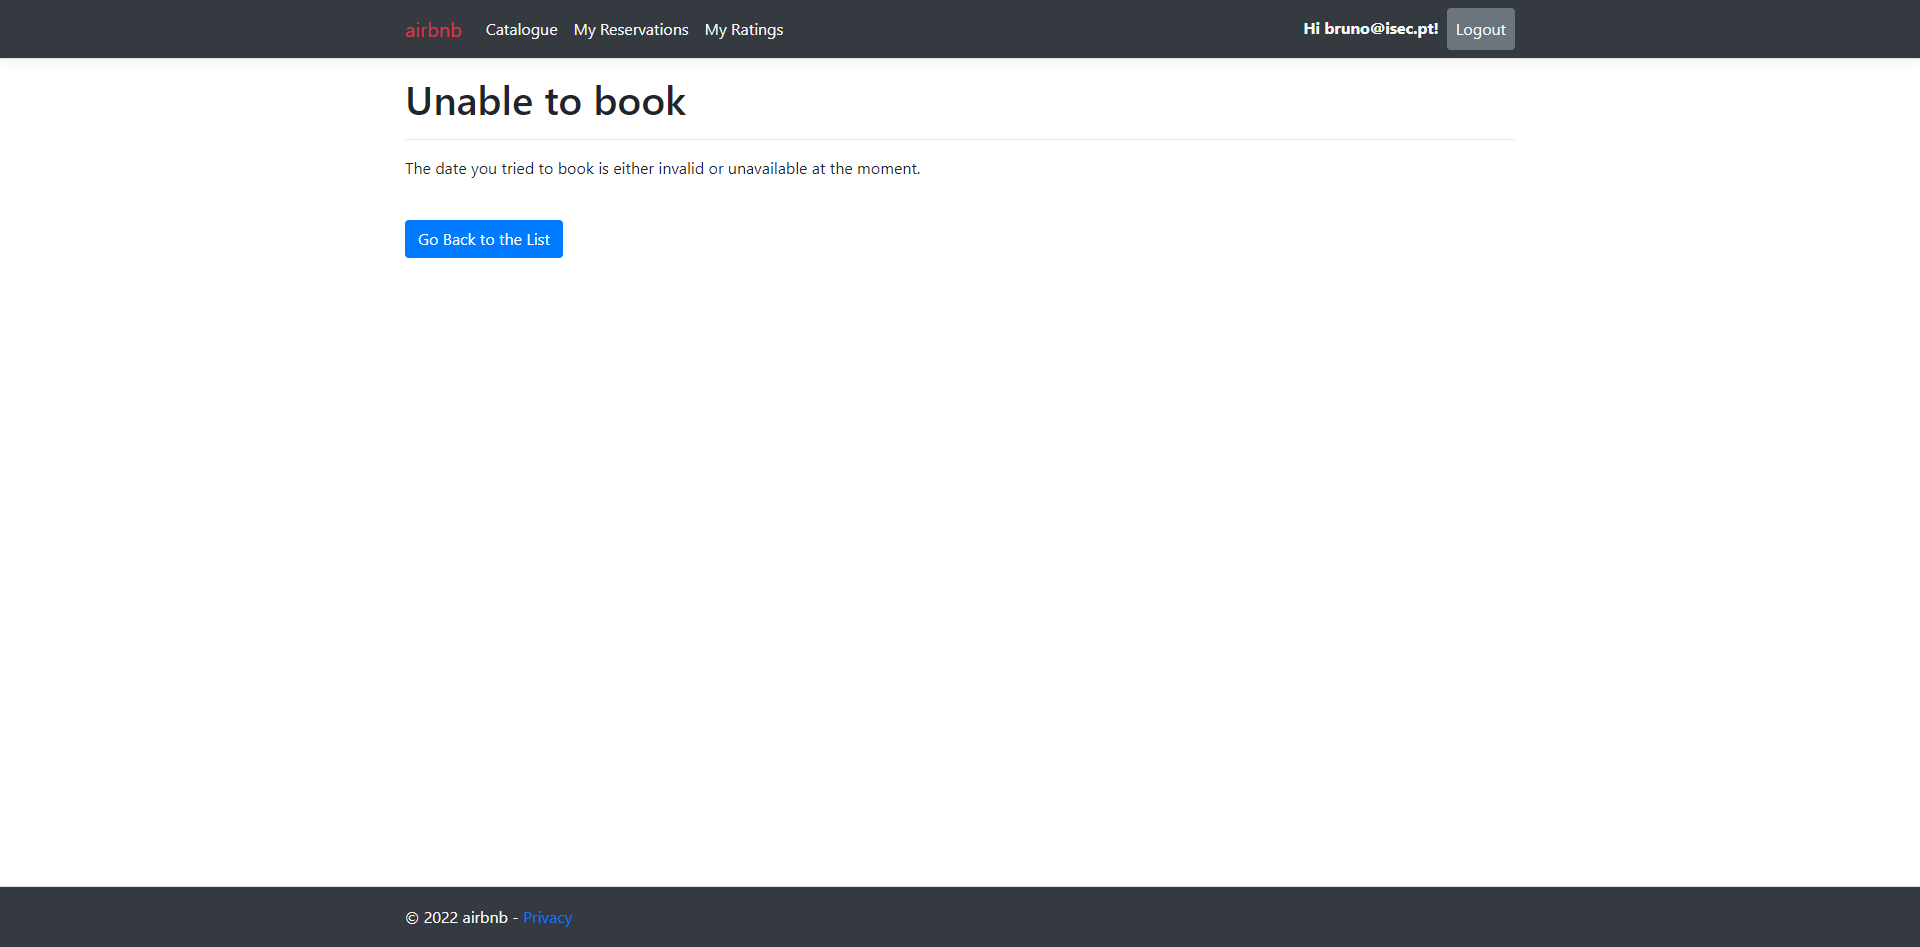
\includegraphics[width=0.95\textwidth,height=0.88\textheight,keepaspectratio]{booking-error-customer}
		\centering
		\caption{Customer - Booking Error}
		\label{fig:customer-booking-error}
	\end{figure}

	\begin{figure}[!ht]
		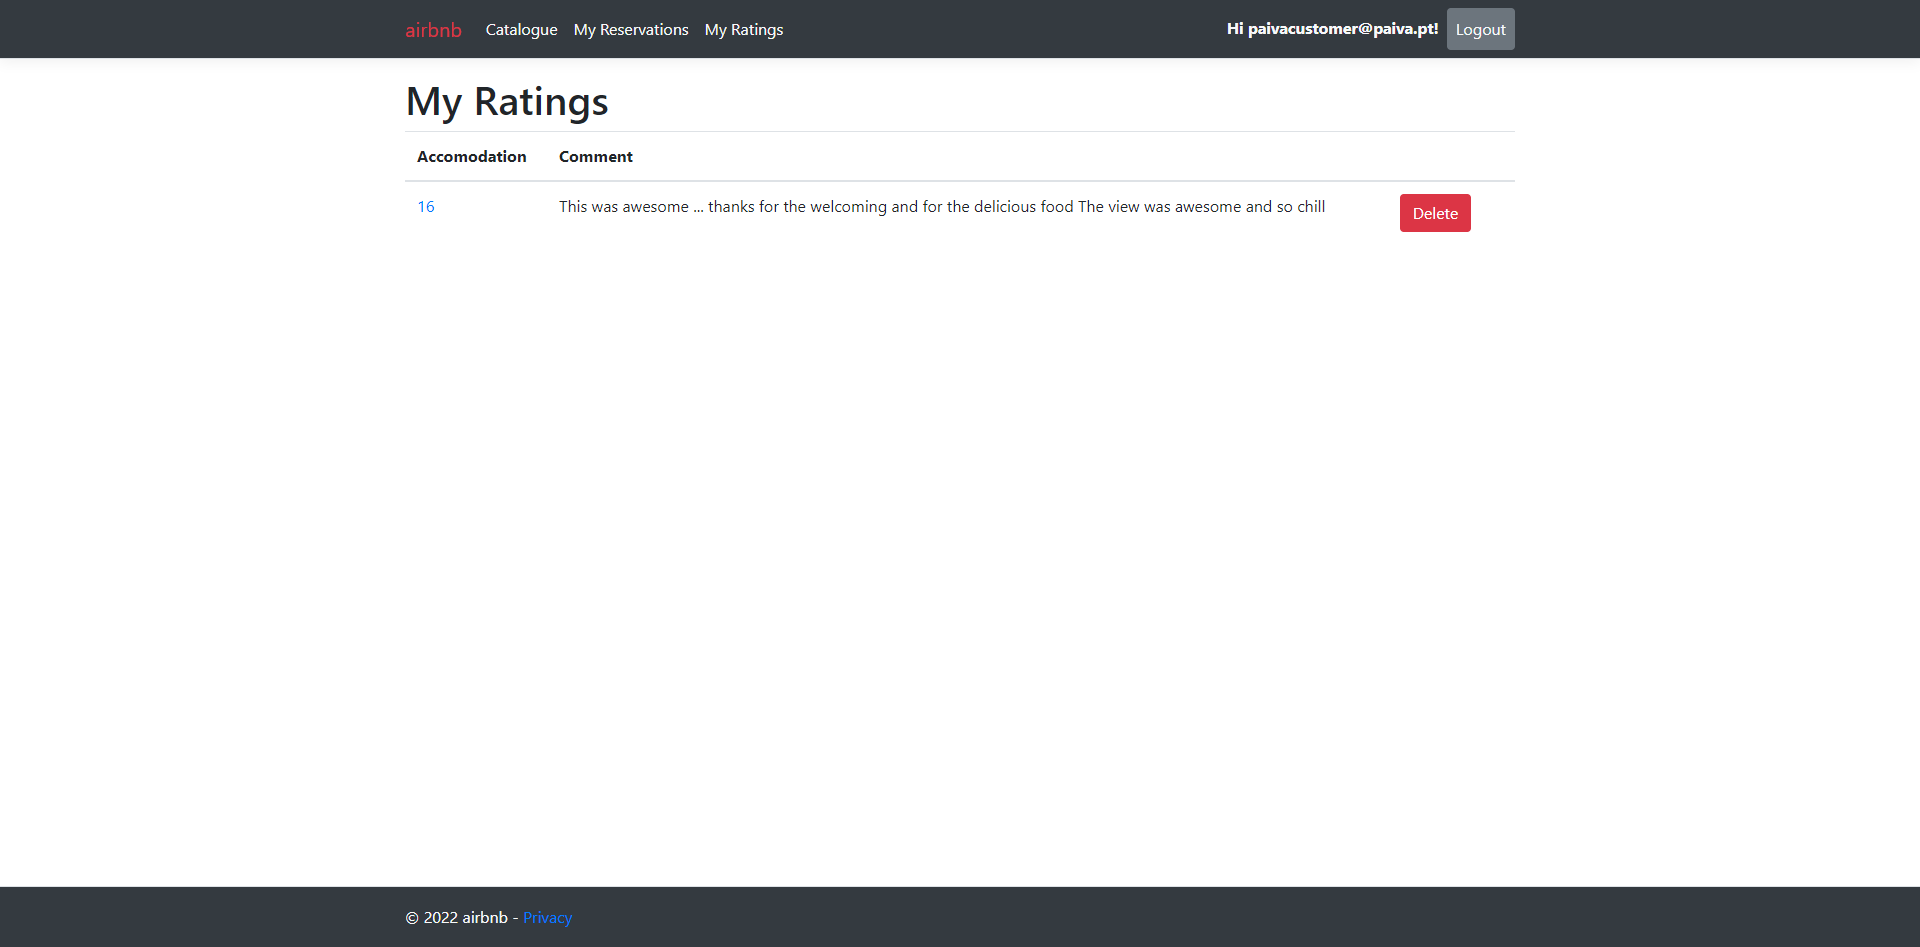
\includegraphics[width=0.95\textwidth,height=0.88\textheight,keepaspectratio]{ratings-customer}
		\centering
		\caption{Customer - Lista de Ratings Que Realizou}
		\label{fig:customer-ratings}
	\end{figure}

	\begin{figure}[!ht]
		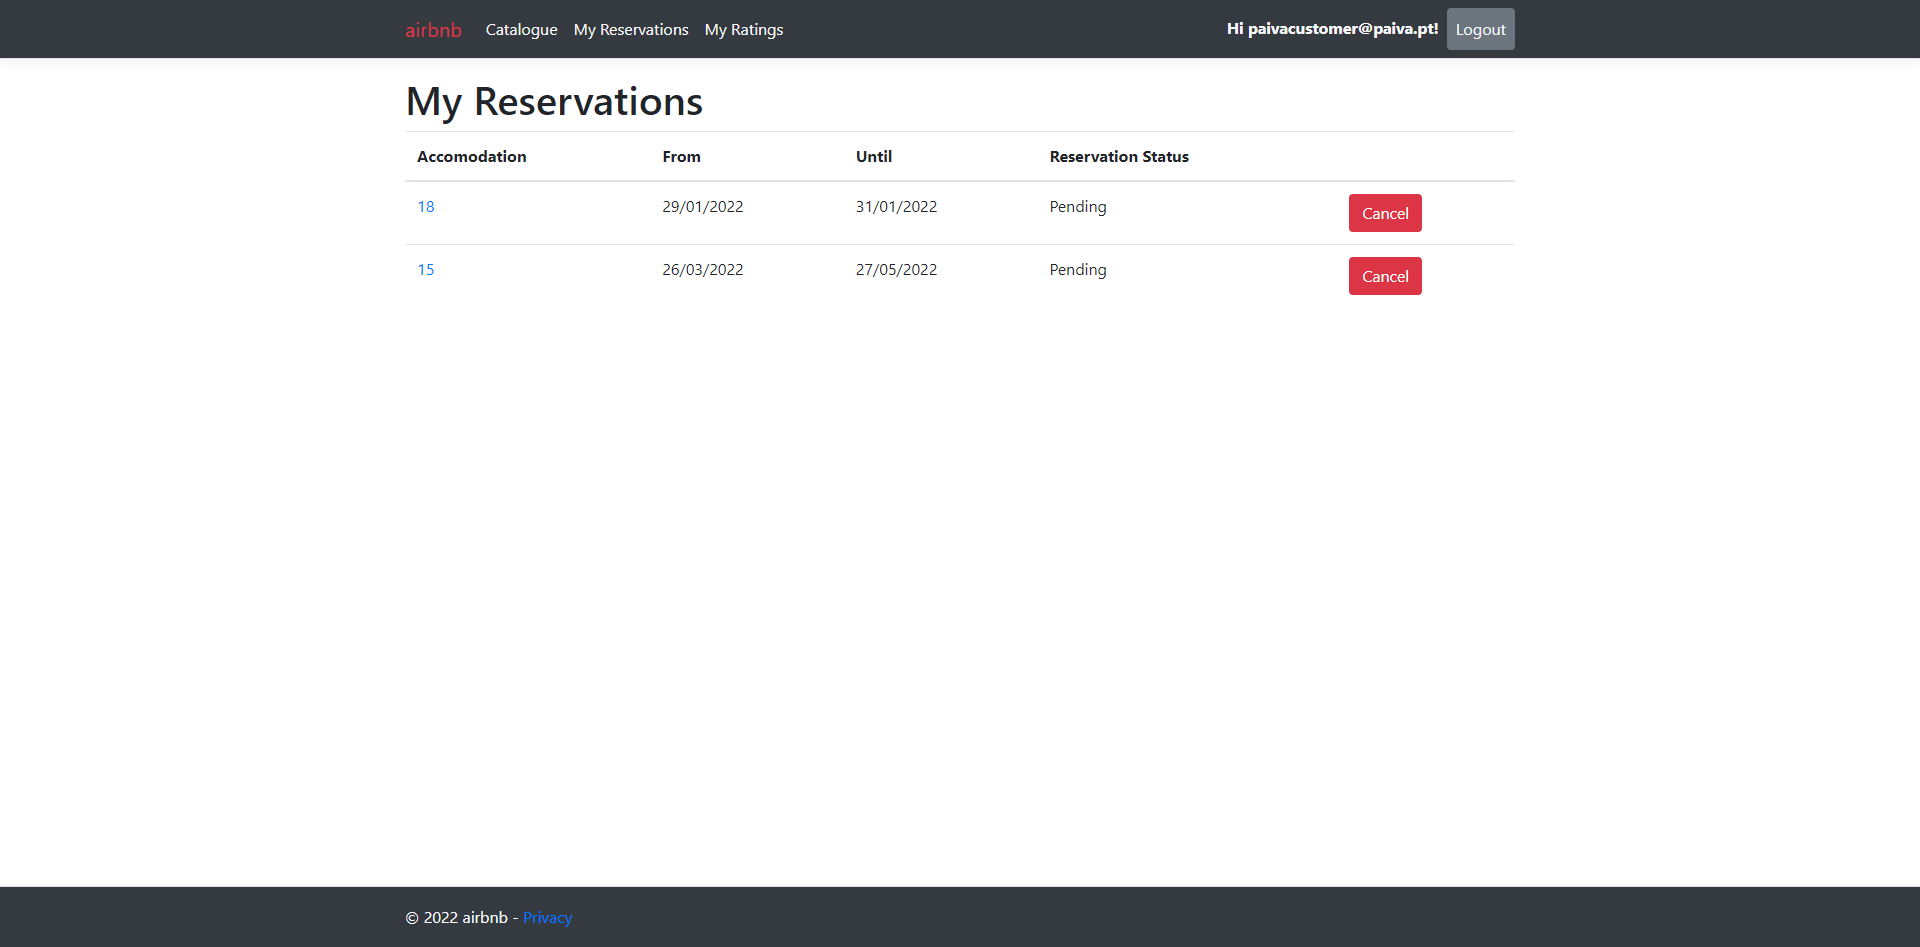
\includegraphics[width=0.95\textwidth,height=0.88\textheight,keepaspectratio]{reservations-customer}
		\centering
		\caption{Customer - Lista de Reservas Que Realizou}
		\label{fig:customer-reservations}
	\end{figure}

	\begin{figure}[!ht]
		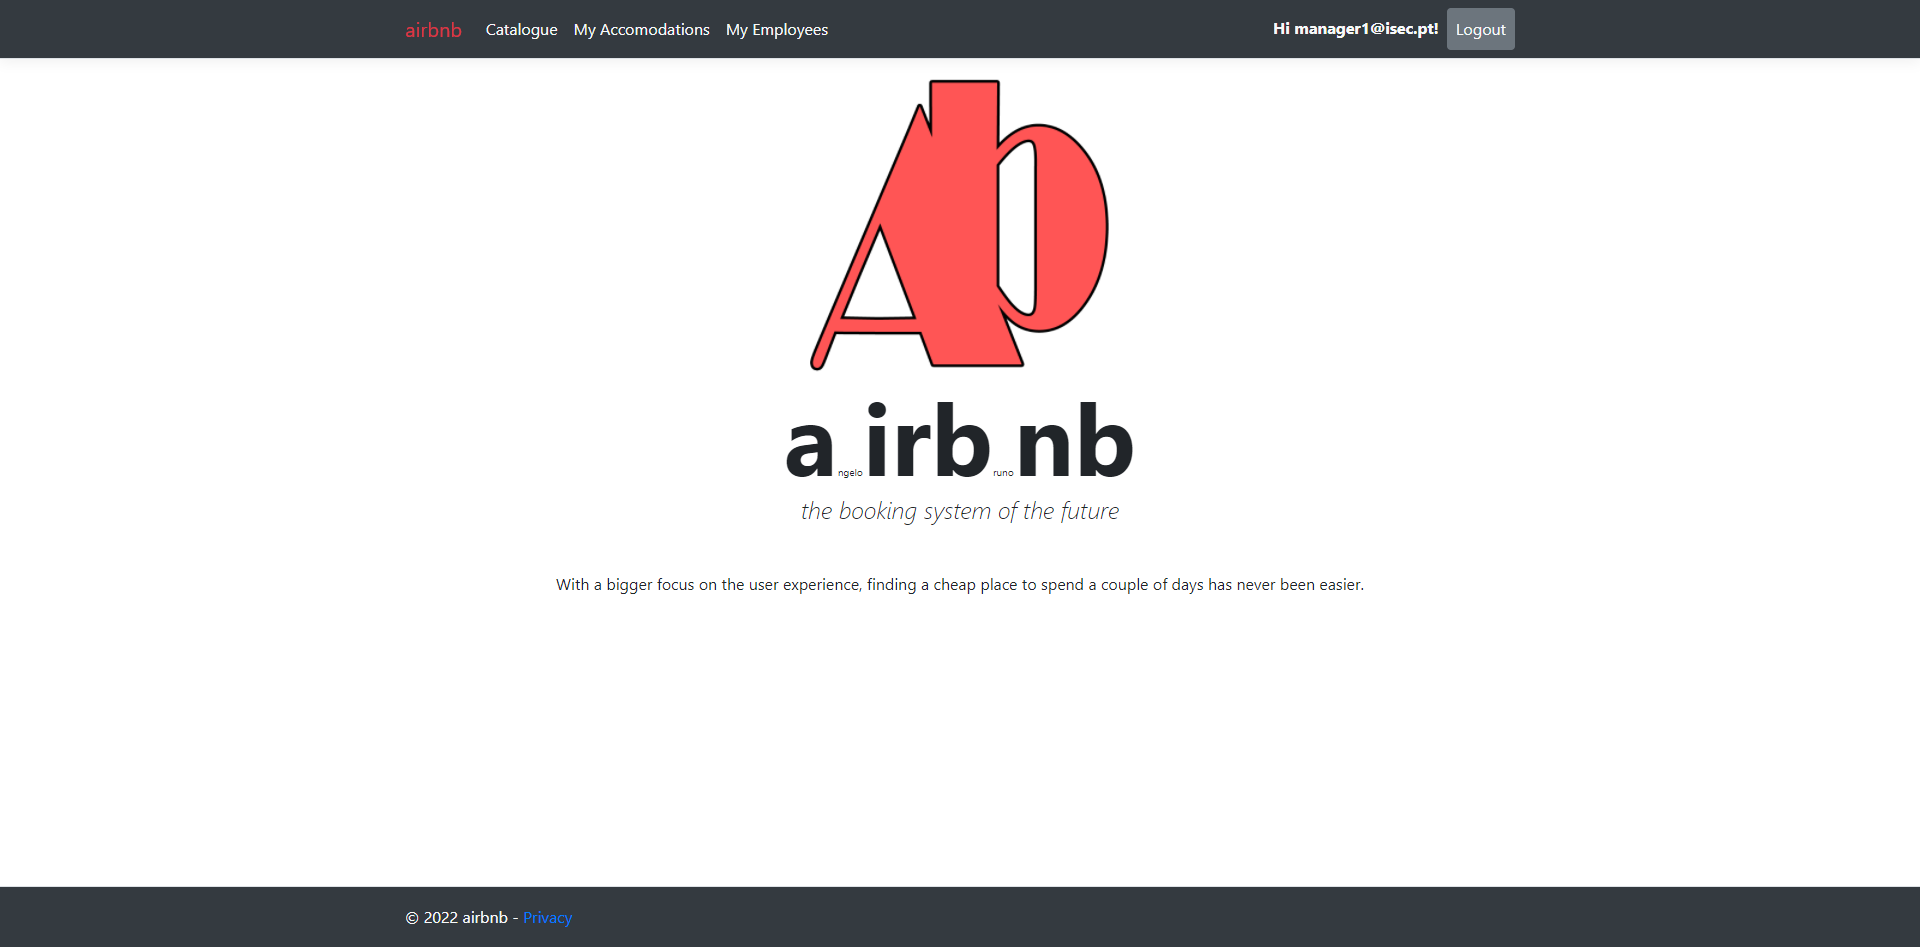
\includegraphics[width=0.95\textwidth,height=0.88\textheight,keepaspectratio]{home-manager}
		\centering
		\caption{Manager - Home Page}
		\label{fig:manager-home-page}
	\end{figure}

	\begin{figure}[!ht]
		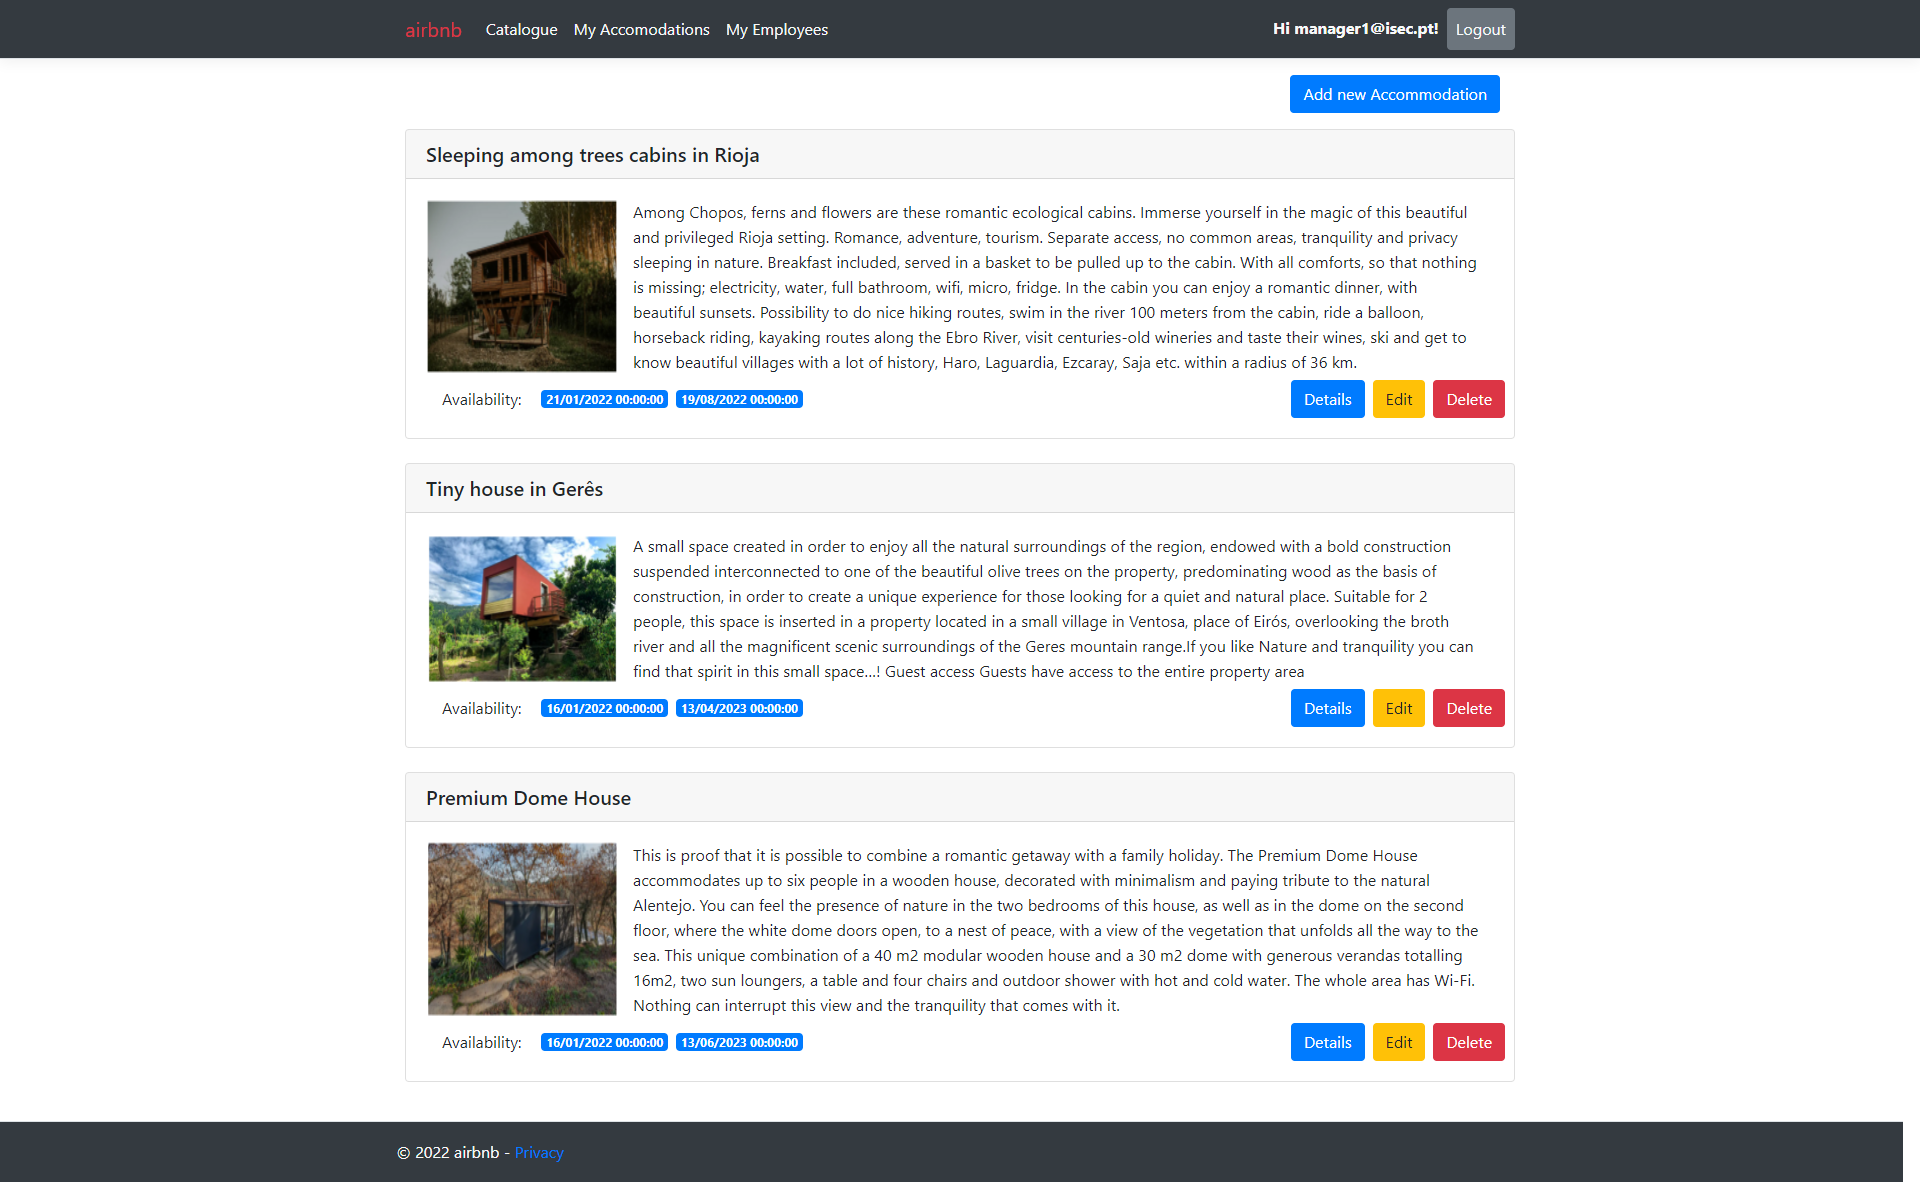
\includegraphics[width=0.95\textwidth,height=0.88\textheight,keepaspectratio]{accommodations-manager}
		\centering
		\caption{Manager - Lista de Acomodações Que Registou no Site}
		\label{fig:manager-accommodations}
	\end{figure}

	\begin{figure}[!ht]
		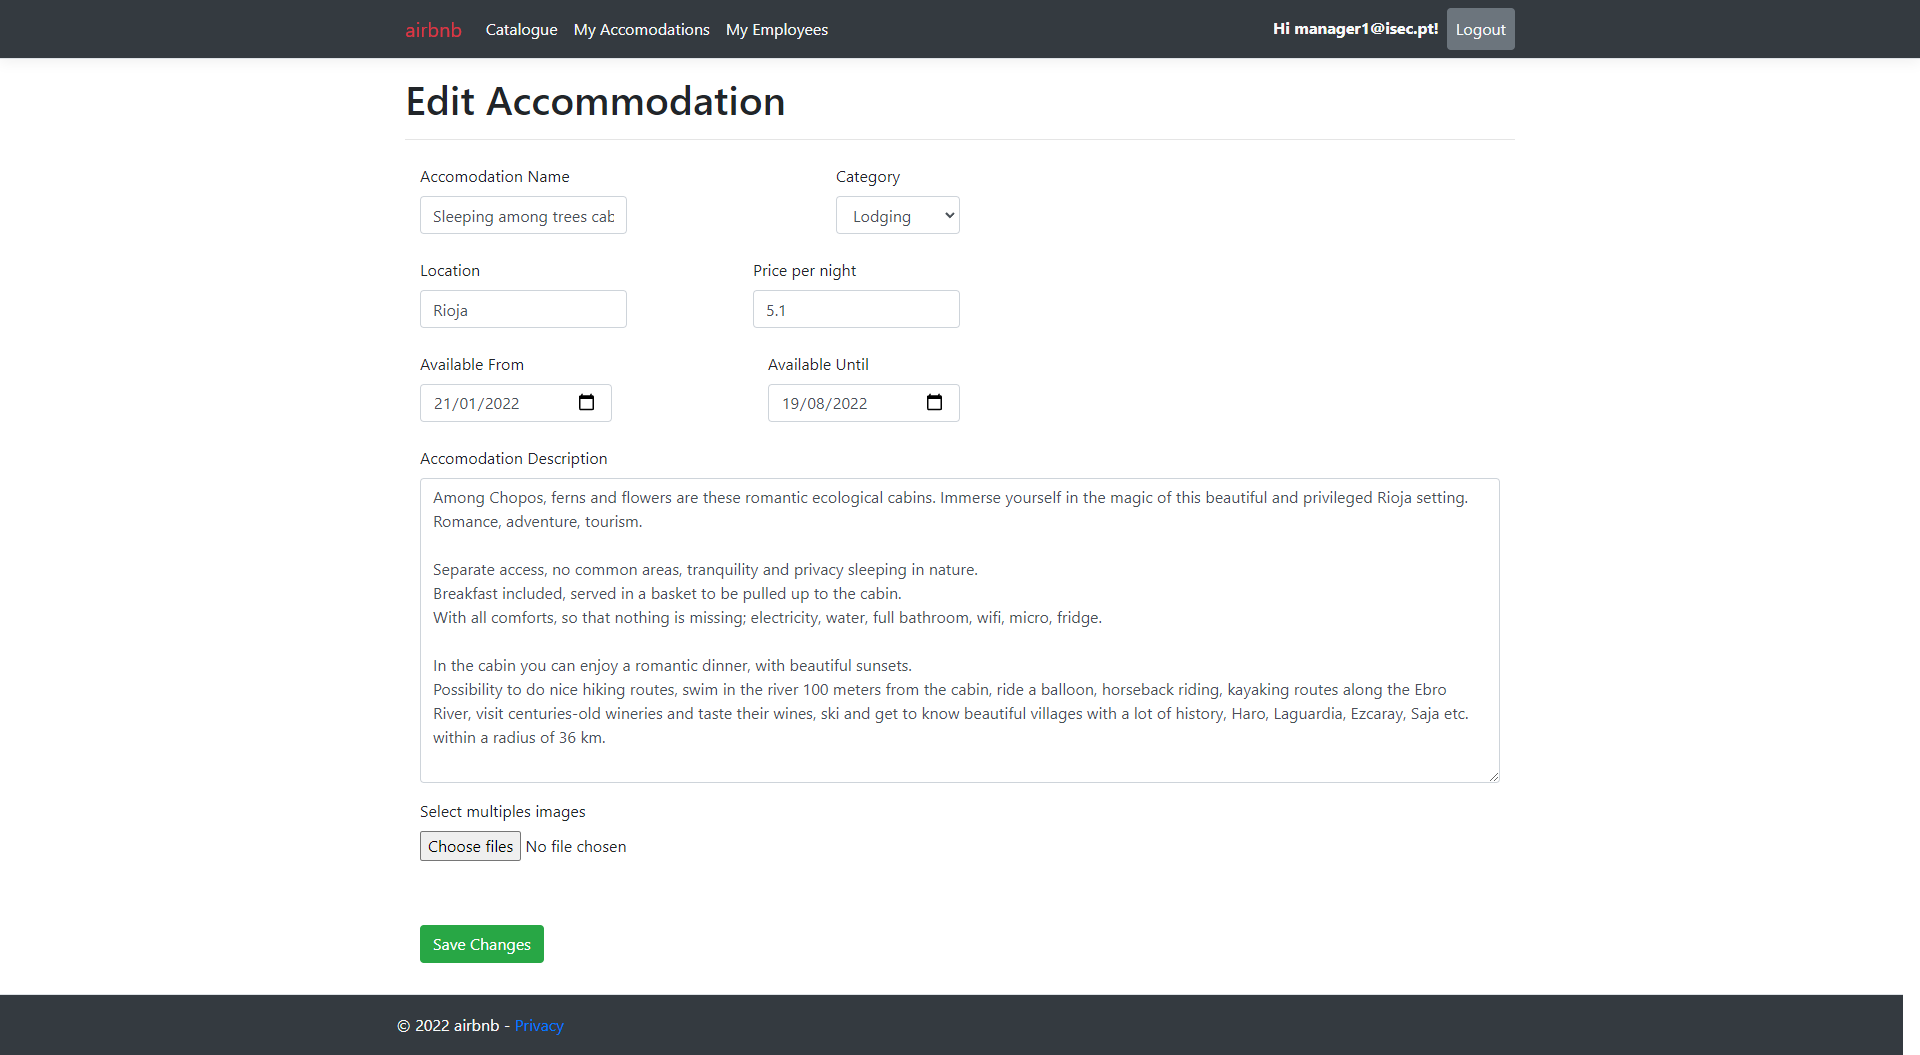
\includegraphics[width=0.95\textwidth,height=0.88\textheight,keepaspectratio]{edit-accommodation-manager}
		\centering
		\caption{Manager - Editar Acomodação}
		\label{fig:manager-edit-accommodation}
	\end{figure}

	\begin{figure}[!ht]
		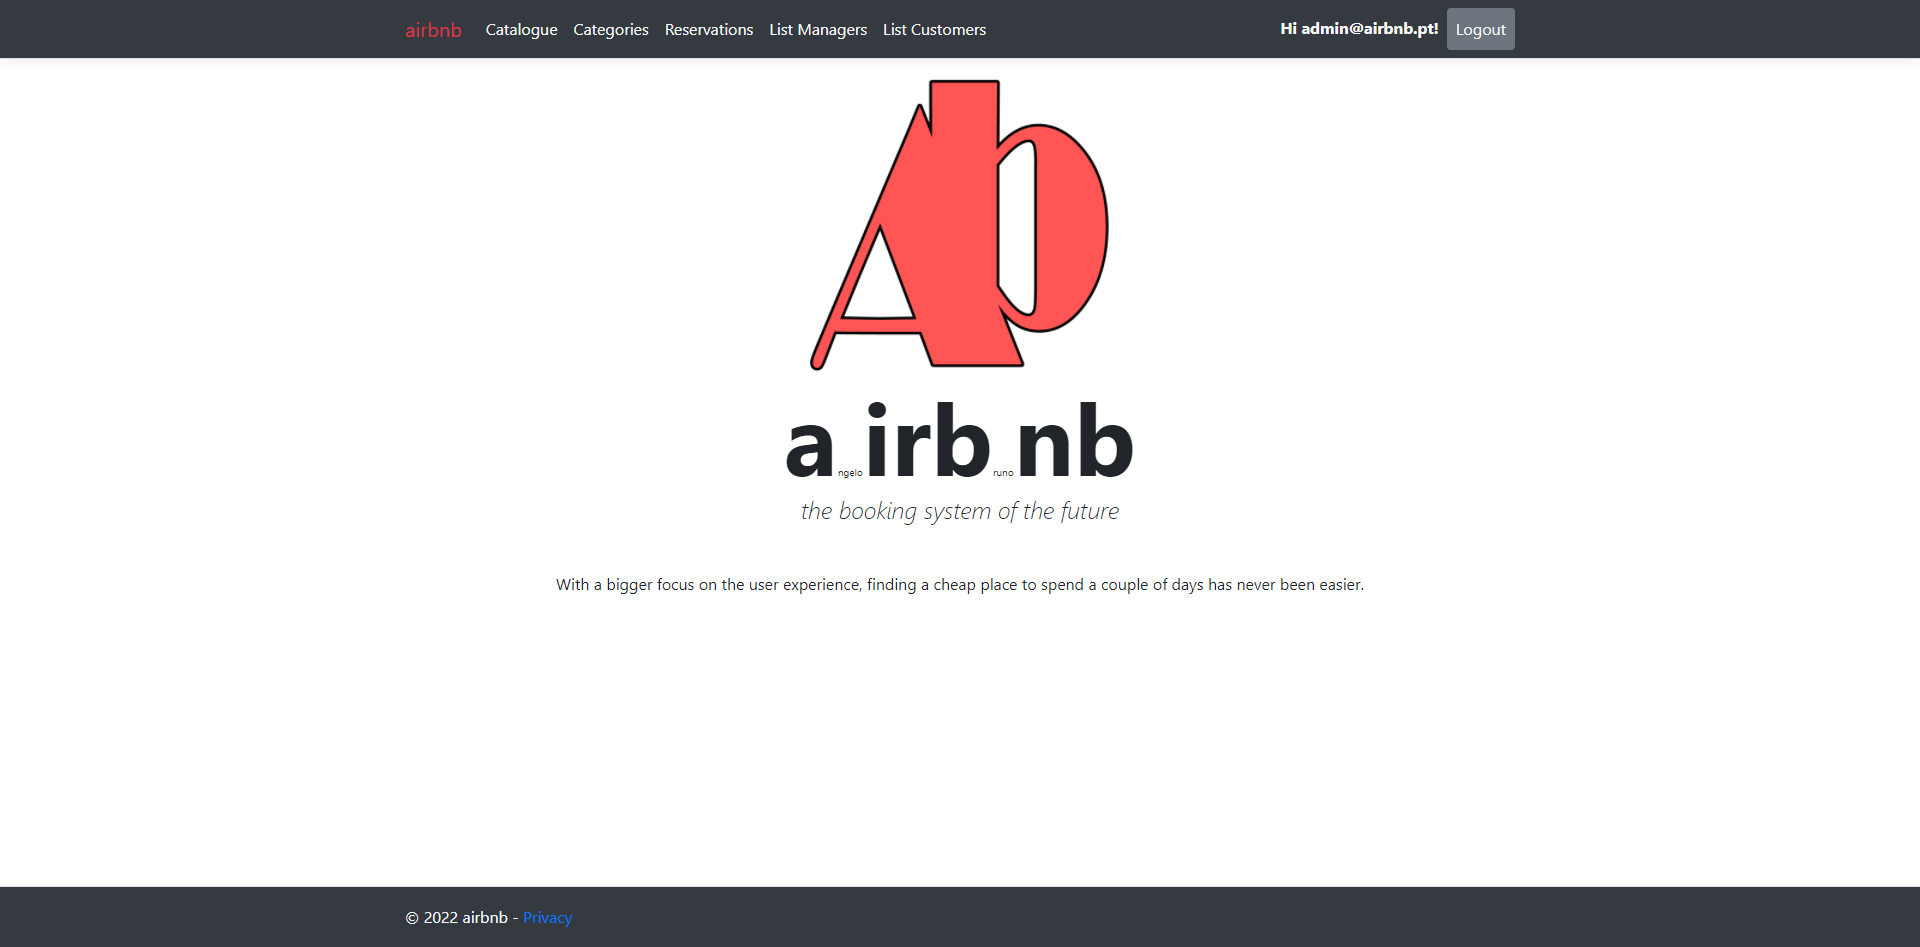
\includegraphics[width=0.95\textwidth,height=0.88\textheight,keepaspectratio]{home-admin}
		\centering
		\caption{Admin - Home Page}
		\label{fig:admin-home-page}
	\end{figure}
	    
    \vfill
    \clearpage
    
    
	\large
	\section{Conclusão}
	\normalsize
	
	Para além de ter sido um verdadeiro desafio, este trabalho foi uma excelente oportunidade para conhecer melhor \textbf{C\#}, \textbf{LINQ} e todas as vantagens que nos proporcionam.
	
	
	\large
	\section{Anexos}
	\normalsize
	
	\listoffigures
\end{document}